%
\section{The Fundamental Data Structures within StdRegions}
\label{sec:stdregions-datastructures}

In almost all object-oriented languages (which includes $C++$), there exists the concepts of {\em class attributes} and {\em object attributes}.  Class attributes are those attributes shared by all object instances (both immediate and derived objects) of a particular class definition, and object attributes (sometimes called data members) are those attributes whose values vary from object to object and hence help to characterize (or make unique) a particular object. In $C++$, object attributes are specified a header file containing class declarations; within a class declaration, attributes are grouped by their accessibility: {\em public} attributes, {\em protected} attributes and {\em private} attributes.  A detailed discussion of the nuances of these
categories are beyond the scope of this guide; we refer the interested reader to the following books for further details:  \cite{BStroustrup,SMeyers}.
For our purposes, the main thing to appreciate is that categories dictate access patters within the inheritance hierarchy and to the ``outside'' world 
(i.e. access from outside the object).  We have summarized the relationships between the categories and their accessibility in Tables
\ref{table:stdreg_publicinheritance}, \ref{table:stdreg_protectedinheritance} and \ref{table:stdreg_privateinheritance} \footnote{These tables are based upon information provided at http://www.programiz.com/cpp-programming/public-protected-private-inheritance, accessed 6 April 2018.}.


\begin{table}[ht]
\begin{center}
\caption{Accessibility in Public Inheritance}
\label{table:stdreg_publicinheritance}
\begin{tabular}{c c c c}
\hline\hline
Accessibility & private variables & protected variables & public variables \\
\hline
Accessibility from own class? & yes & yes & yes \\
Accessibility from derived class? & no & yes & yes\\
Accessibility from 2nd derived class? & no & yes & yes\\
\end{tabular}
\end{center}
\end{table}

\begin{table}[ht]
\begin{center}
\caption{Accessibility in Protected Inheritance}
\label{table:stdreg_protectedinheritance}
\begin{tabular}{c c c c}
\hline\hline
Accessibility & private variables & protected variables & public variables \\
\hline
Accessibility from own class? & yes & yes & yes \\
Accessibility from derived class? & no & yes & yes \\
&&&(inherited as \\
&&&protected variable)\\
Accessibility from 2nd derived class? & no & yes & yes\\
\end{tabular}
\end{center}
\end{table}

\begin{table}[ht]
\begin{center}
\caption{Accessibility in Private Inheritance}
\label{table:stdreg_privateinheritance}
\begin{tabular}{c c c c}
\hline\hline
Accessibility & private variables & protected variables & public variables \\
\hline
Accessibility from own class? & yes & yes & yes\\
Accessibility from derived class? & no & yes & yes \\
& & (inherited as & (inherited as \\
& & private variable) &  private variable) \\
Accessibility from 2nd derived class? & no & no & no \\
\end{tabular}
\end{center}
\end{table}

Within the StdRegions directory of the library, there exists a class inheritance hierarchy designed to try to encourage re-use of core
algorithms (while simultaneously trying to minimize duplication of code).  We present this class hierarchy in Figure \ref{stdregions:stdexpansiontree}.

\begin{figure}[htb]
\centering
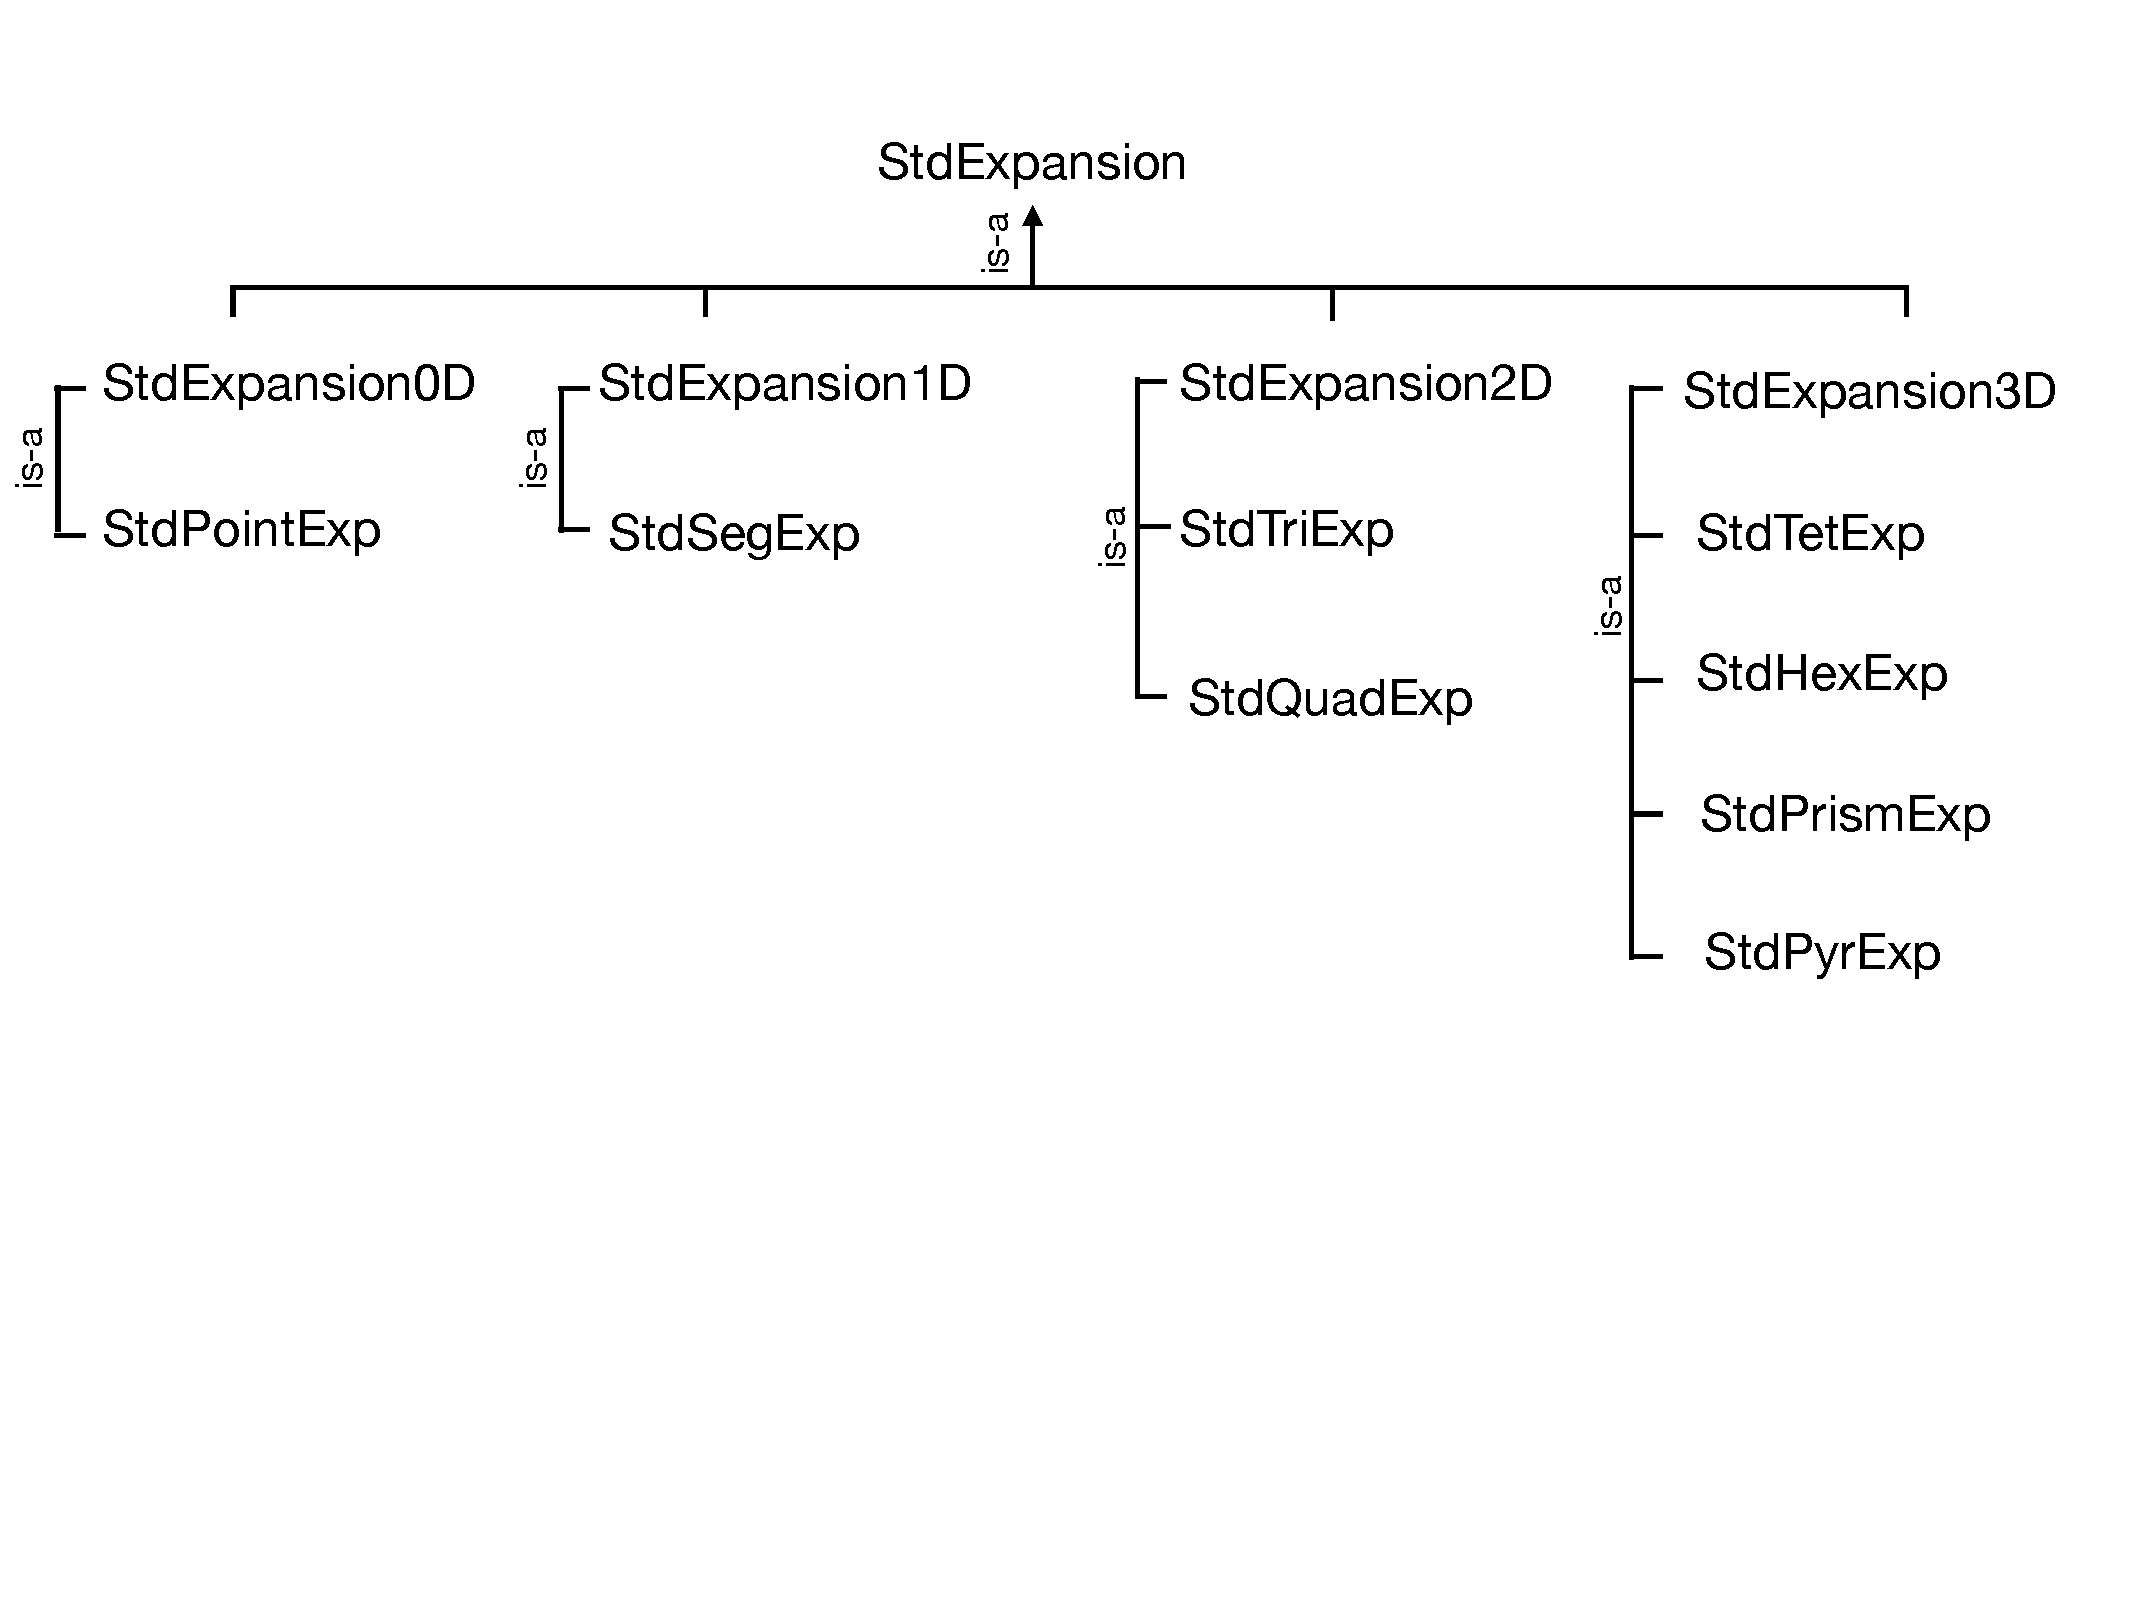
\includegraphics[width=6in]{img/stdexpansiontree.pdf}
\caption{Class hierarchy derived from StdExpansion, the base class of the StdRegions Directory.}
\label{stdregions:stdexpansiontree}
\end{figure}

As is seen in Figure \ref{stdregions:stdexpansiontree}, the StdRegions hierarchy consists of three levels:  the base level from which all
StdRegion objects are derived is StdExpansion.   This object is then specialized by dimension, yielding StdExpansion0D, 
StdExpansion1D, StdExpansion2D and StdExpansion3D.  The dimension-specific objects are then specialized based upon
shape.  

The object attributes (variables) at various levels of the hierarchy can be understood in light of Figure \ref{stdregions:stdexpansion}.
At its core, an expansion is a means of representing a function over a canonically-defined region of space evaluated at a collection of point positions.
The various data members hold information to allow all these basic building blocks to be specified.

\begin{figure}[htb]
\centering
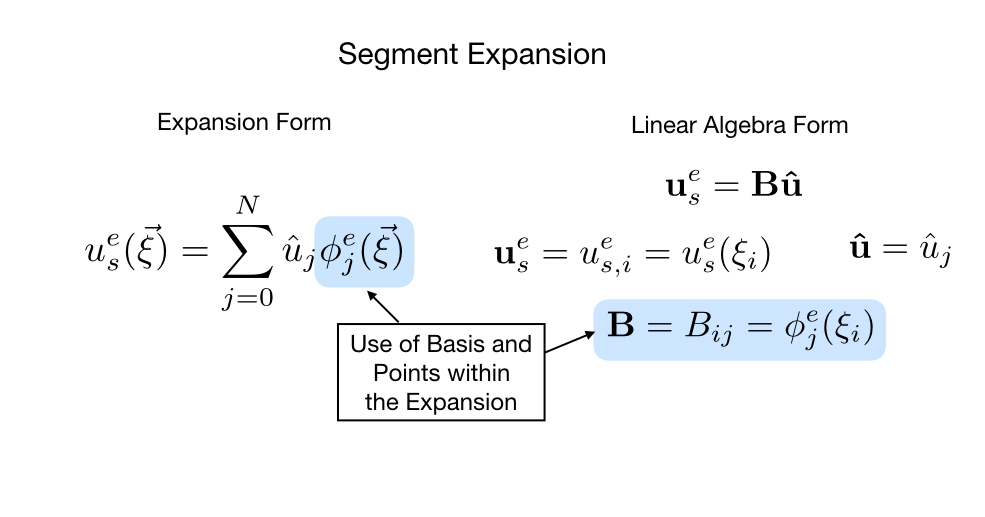
\includegraphics[width=6in]{img/StdExpansion.png}
\caption{Diagram to help understand the various data members (object attributes) contained within StdRegions and how they connect with the mathematical representation presented earlier.}
\label{stdregions:stdexpansion}
\end{figure}

The various private, protected and public data members contained within StdRegions are provided in the subsequent sections.

%%%%%%%%%%%%%%%%%%%%%%%%%%%%%%%%%%%%%%%%
\subsection{Variables at the Level of StdExpansion}

\paragraph{Private:}

There are private methods but no private data members within StdExpansion.

\paragraph{Protected:}

\begin{itemize}
\item  Array of Basis Shared Pointers:  \verb+m_base+
% 
\item  Integer element id: \verb+m_elmt_id+
%
\item Integer total number of coefficients in the expansion:  \verb+m_ncoeffs+
%
\item Matrix Manager: \verb+m_stdMatrixManager+
%
\item Matrix Manager: \verb+m_stdStaticCondMatrixManager+
%
\item IndexKeyMap Matrix Manager: \verb+m_IndexMapManager+
\end{itemize}


\paragraph{Public:}

There are public methods but no public data members within StdExpansion.



%%%%%%%%%%%%%%%%%%%%%%%%%%%%%%%%%%%%%%%%
\subsection{Variables at the Level of StdExpansion\$D for various Dimensions}

\paragraph{Private:}

There are private methods but no private data members within StdExpansion\$D.

\paragraph{Protected:}


\begin{itemize}
\item 0D and 1D: std::map<int, NormalVector> \verb+m_vertexNormals+
%
\item 2D: Currently does not have any data structure.  It should probably have \verb+m_edgeNormals+
%
\item 3D: std::map<int, NormalVector> \verb+m_faceNormals+
%
\item 3D: std::map<int, bool> \verb+m_negatedNormals+
\end{itemize}

\paragraph{Public:}

There are public methods but no public data members within StdExpansion\$D.

%%%%%%%%%%%%%%%%%%%%%%%%%%%%%%%%%%%%%%%%
\subsection{Variables at the Level of Shape-Specific StdExpansions}

\paragraph{Private:}

\paragraph{Protected:}

\paragraph{Public:}


%%%%%%%%%%%%%%%%%%%%%%%%%%%%%%%%%%%%%%%%
\subsection{General Layout of the Basis Functions in Memory}

\subsection{General Layout}

Basis functions are stored in a 1D array indexed by both mode and quadrature point. The fast index runs over quadrature points while the slow index runs over modes. This was done to match the memory access pattern of the inner product, which is the most frequently computed kernel for most solvers.

Bases are built from the tensor product of three different equation types (subsequently called Type 1, Type II and Type III respectively):
\begin{equation}
    \phi_{p}(z) =
    \begin{cases}
        \frac{1 - z}{2} & p = 0 \\
        \frac{1 + z}{2} & p = 1 \\
        \left(\frac{1-z}{2}\right)\left(\frac{1+z}{2}\right) P_{p-1}^{1,1}(z) & 2 \leq p < P
    \end{cases}
\end{equation}

\[
    \phi_{pq}(z) = \left\{
    \begin{array}{lll}
        \phi_{q}(z) & p = 0 & 0 \leq q < P \\
        \left(\frac{1 - z}{2}\right)^p & 1 \leq p < P & q = 0 \\
        \left(\frac{1-z}{2}\right)^p \left(\frac{1+z}{2}\right) P_{q-1}^{2p-1,1}(z) & 1 \leq p < P, & 1 \leq q < P - p
    \end{array}\right.
\]

\[
    \phi_{pqr}(z) = \left\{
    \begin{array}{llll}
        \phi_{qr} & p = 0 & 0 \leq q < P & 0 < r < P - q \\
        \left(\frac{1-z}{2}\right)^{p+q} & 1 \leq p < P, & 0 \leq q < P - p, & r = 0 \\
        \left(\frac{1 - z}{2}\right)^{p + q} \left(\frac{1+z}{2}\right) P_{r-1}^{2p + 2q - 1, r}(z) & 1 \leq p < P, & 0 \leq q < P - p, & 1 \leq r < P - p - qr.
    \end{array}\right.
\]

Here, $P$ is the polynomial order of the basis and $P^{\alpha,\beta}_{p}$ are the $p^{\text{th}}$ order jacobi polynomial.

\subsubsection{A Note Concerning Adjustments For $C_0$ Continuity}


Before going further it is worth reviewing the spatial shape of each node. The term $\frac{1 + z}{2}$ is an increasing function which is equal to zero at $z = -1$ and equal to one at $z = 1$. Similarly, $\frac{1 - z}{2}$ is a decreasing function which is equal to one at $z = -1$ and equal to zero at $z = +1$. These two functions are thus non-zero at one of each of the boundaries. If we need to maintain $C_0$ continuity with surrounding elements (as we do in the continuous Galerkin method), then these local modes must be assembled together with the correct local modes in adjacent elements to create a continuous, global mode. For instance $\frac{1 + z}{2}$ in the left element would be continuous with $\frac{1 - z}{2}$ in the right element. The union of these two modes under assembly form a single ``hat'' function. By contrast, functions of the form
\[
    \frac{1 - z}{2} \frac{1 + z}{2}
\]
are zero at both end points $z = \pm 1$. As a result, they are trivially continuous with any other function which is also equal to zero on the boundary. These ``bubble'' functions may be treated entirely locally and thus are used to construct the interior modes of a basis. Only bases with $p > 1$ have interior modes.

All of this holds separately in one dimension. Higher dimensional bases are constructed via the tensor product of 1D basis functions. As a result, we end up with a greater number of possibilities in terms of continuity. When the tensor product is taken between two bubble functions from different bases, the result is still a bubble function. When the tensor product is taken between a hat function and a bubble function we get ``edge'' modes (in both 2D and 3D). These are non-zero along one edge of the standard domain and zero along the remaining edges. When the tensor product is taken between two hat functions, they form a ``vertex'' mode which reaches its maximum at one of the vertices and is non-zero on two edges.  The 3D bases are constructed similarly.

Based upon this convention, the 1D basis set consists of vertex modes and bubble modes.  The 2D basis function set consists of vertex modes, edge modes and bubble modes.  The 3D basis set contains vertex modes, edge modes, face modes and bubble modes.

\subsection{2D Geometries}

\subsubsection{Quadrilateral Element Memory Organization}
Quads have the simplest memory organization. The quadrilateral basis is composed of the tensor product of two Type I functions $\phi_p(\xi_{0,i}) \phi_q(\xi_{1,j})$. This function would then be indexed as

\begin{lstlisting}
    basis0[p*nq0 + i] * basis1[q*nq1 + j]
\end{lstlisting}
where nq<b> is the number of quadrature points for the $b^{\text{th}}$ basis. Unlike certain mode orderings (e.g. Karniadakis and Sherwin \cite{KaSh05}), the two hat functions are accessed as the first and second modes in memory with interior modes placed afterward. Thus,
\begin{lstlisting}
    basis[i], basis[nq + i]
\end{lstlisting}
correspond to $\frac{1 - z}{2}$ and $\frac{1 + z}{2}$ respectively.

\subsubsection{Triangle Element Memory Organization}
Due to the use of collapsed coordinates, triangular element bases are formed via the tensor product of one basis function of Type I, and one of Type II, i.e. $\phi_p(\eta_{0,i} \phi_pq(\eta{1,j}))$. Since $\phi_p$ is also a Type I function, its memory ordering is identical to that used for quads. The second function is complicated by the mixing of $\xi_0$ and $\xi_1$ in the construction of $\eta_1$.

In particular, this means that the basis function has two modal indices, $p$ and $q$. While $p$ can run all the way to $P$, The number of $q$ modes depends on the value of the $p$ index q index such that $0 \leq q < P - p$. Thus, for $p = 0$, the q index can run all the way up to $P$. When p = 1, it runs up to $P - 1$ and so on. Memory is laid out in the same way starting with $p=0$. To access all values in order, we write
\begin{lstlisting}
    mode = 0
    for p in P:
        for q in P - p:
            out[mode*nq + q] = basis0[p*nq]*basis1[mode*nq + q]
        mode += P-p
\end{lstlisting}
Notice the use of the extra ``mode'' variable. Since the maximum value of $q$ changes with $p$, basis1 is not simply a linearized matrix and instead has a triangular structure which necessitates keeping track of our current memory location.

The collapsed coordinate system introduces one extra subtlety. The mode
\[
    \phi_1(\eta_1) \phi_1(\eta_2)
\]
represents the top right vertex in the standard basis. However, when we move to the standard element basis, we are dealing with a triangle which only has three vertices. During the transformation, the top right vertex collapses into the top left vertex. If we naively construct an operators by iterating through all of our modes, the contribution from this vertex to mode $\Phi_{01}$ will not be included. To deal with this, we add its contribution as a correction when computing a kernel. The correction is $\Phi_{01} = \phi_0 \phi_{01} + \phi_1 \phi_{10}$ for a triangle.

\subsection{3D Geometries}

\subsubsection{Hexahedral Element Memory Organization}
The hexahedral element does not differ much from the quadrilateral as it is the simply the product of three Type I functions.
\[
    \Phi_{pqr} = \phi_p(\xi_0) \phi_q(\xi_1) \phi_r(\xi_2).
\]

\subsubsection{Prismatic Element Memory Organization}
Cross sections of a triangular prism yield either a quad or a triangle based chosen direction. The basis, therefore, looks like a combination of the two different 2D geometries.
\[
    \Phi_{pqr} = \phi_p(\eta_0)\phi_q(\xi_1)\phi_{pr}(\eta_1).
\]
Taking $\phi_p \phi_{pr}$ on its own produces a triangular face while taking $\phi_p \phi_q$ on its own produces a quadrilateral face. When the three basis functions are combined into a single array (as in the inner product kernel), modes are accessed in the order p,q,r with r being the fastest index and p the slowest. The access pattern for the prism thus looks like
\begin{lstlisting}
    mode_pqr = 0
    mode_pr = 0
    for p in P:
        for q in Q:
            for r in P - p:
                out[mode_pqr*nq + r] = basis0[p*nq]*basis1[q*nq]*basis2[mode_pr + r]
            mode_pqr += P - p
        mode_pr += P - p
\end{lstlisting}

As with the triangle, we have to deal with complications due to collapsed coordinates. This time, the singular vertex from the triangle occurs along an entire edge of the prism. Our correction must be added to a collection of modes indexed by $q$
\[
    \Phi_{0q1} += \phi_1 \phi_q \phi_{10}.
\]

\subsubsection{Tetrahedral Element Memory Organization}
The tetrahedral element is the most complicated of the element constructions. It cannot simply be formed as the composition of multiple triangles since $\eta_2$ is constructed by mixing three coordinate directions. We thus need to introduce our first Type III function.
\[
    \Phi_{pqr}(\eta_0, \eta_1, \eta_2) = \phi_{p}(\eta_0) \phi_{pq} (\eta_1) \phi_{pqr}(\eta_2).
\]
The $r$ index is constrained by both $p$ and $q$ indices. It runs from $P - p - q$ to $1$ in a similar manner to the Type II function. Our typical access pattern is thus
\begin{lstlisting}
mode_pqr = 0
mode_pq = 0
for p in P:
    for q in P - p:
        for r in P - p - r:
            out[mode_pqr*nq + r] = basis0[p*nq]*basis1[mode_pq + q]*basis2[mode_pqr + r]
        mode_pqr += (P - p - r)
    mode_pq += (P - p)
\end{lstlisting}
The tetrahedral element also has to add a correction due to collapsed coordinates. Similar to the prism, the correction must be applied to an entire edge indexed by $r$
\[
    \Phi_{01r} += \phi_1 \phi_1 \phi_{11r}.
\]

\subsubsection{Pyramidic Element Memory Organization}
Like the tetrahedral element, a pyramid contains a collapsed coordinate direction which mixes three standard coordinates from the standard region. Unlike the tetrahedra, the collapse only occurs along one axis. Thus it is constructed from two Type I functions and one Type III function
\[
    \Phi_{pqr} = \phi_p(\eta_1) \phi_q(\eta_2) \phi_{pqr}(\eta_3).
\]
The product $\phi_p \phi_q$ looks like the a quad construction which reflects the quad which serves as the base of the pyramid. A typical memory access looks like
\begin{lstlisting}
mode_pqr = 0
for p in P:
    for q in P - p:
        for r in P - p - r:
            out[mode_pqr*nq + r] = basis0[p*nq]*basis1[q*nq]*basis2[mode_pqr*nq + r]
        mode_pqr += (P - p - r)
\end{lstlisting}


